\chapter{Probability Rules}
\section{General Rules}
Here are a few basic rules of probabilities. They should be relatively straightforward.
\begin{theorem}
For a sample space, \sS, the probability of a simple event in \sS~occurring is 1. That is
\[
    P(\sS) = 1
\]
\end{theorem}
\begin{proof}
\[
    P(\sS) = \sum_{a \in \sS} P(a) = \sum_{\all a} P(a)
\]
\end{proof}
\begin{theorem}
Any event $A$ in a sample space has a probability between 0 and 1 inclusive. That is
\[
    0 \leq P(A) \leq 1 \for\all A\subseteq\sS
\]
\end{theorem}
\begin{proof}
Note that $A$ is a subset of \sS, so
\[
    P(A) = \sum_{a \in A} P(a) \leq \sum_{a \in \sS} P(a) = 1
\]
Now, recall that $P(a) \geq 0$ for any sample point $a$ by our probability model. Thus, since $P(A)$ is the sum of non-negative real numbers, $P(A) \geq 0$. So we have
\[
    1 \leq P(A) \leq 1
\]
\end{proof}
\begin{theorem}
If $A$ and $B$ are two events such that $A \subseteq B$, that is all the sample points in $A$ are also in $B$, then 
\[
    P(A) \leq P(B)
\]
\end{theorem}
\begin{proof}
\[
    P(A) = \sum_{a \in A} P(a) \leq \sum_{a \in B} P(a) = P(B)
\]
\end{proof}
% ------------------------------------------------- %
\section{Venn Diagrams}
As we have seen already, it is helpful to think of events in a sample space as subsets of the sample space. Consider a sample space, $\sS = \{\, 1,2,3,4,5,6 \,\}$. A number is picked at random, let $E$ be the event that the number is even. We can think of $E$ as the subsets of \sS, $\{\, 2,4,6 \,\}$ and the probability of $E$ is the probability of any sample points in $A$ occurs, that is 2, 4, or 6 is selected. We can represent the relationships of events in the sample space using Venn diagrams.
\par\smallskip
\begin{figure}[h]
\centering
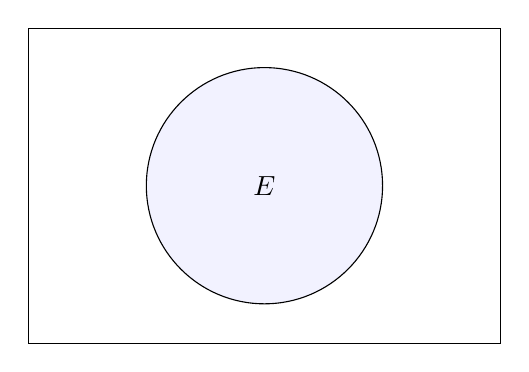
\begin{tikzpicture}
\draw (0,0) rectangle (6,4) node[below left] {$\sS$};
\filldraw[fill=blue!5] (3,2) circle (1.5) node {$E$};
\end{tikzpicture}
\caption{Single event $E$} \label{fig:Single event}
\end{figure}
Now, assuming the area of $E$ is half the area of \sS, we have that the probability of $E$ is the probability that a randomly chosen point on the area of \sS~will be within $E$.

Consider now we let $G = \{\, 4,5,6 \,\}$ be the event that that the number selected is greater than or equal to 4. We have
\par\smallskip
\begin{figure}[h]
\centering
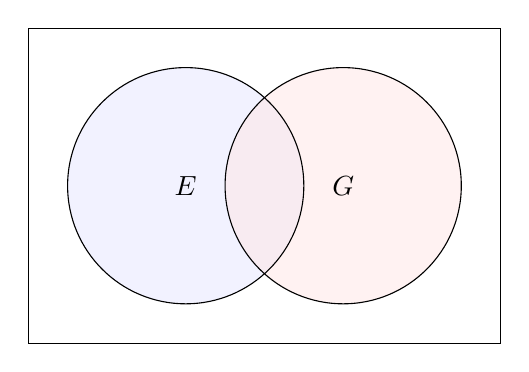
\begin{tikzpicture}

\def\eventE{(2,2) circle (1.5)}
\def\eventG{(4,2) circle (1.5)}

\draw (0,0) rectangle (6,4) node[below left] {$\sS$};

\begin{scope}[fill opacity=0.5]
\fill[blue!10] \eventE;
\fill[red!10] \eventG;
\end{scope}

\draw \eventE node {$E$};
\draw \eventG node {$G$};

\end{tikzpicture}
\caption{Events $E$ and $G$} \label{fig:Events E and G}
\end{figure}
The total shaded region of the Venn diagram, $E \union G$, contains all the sample points of $E$ and $G$. It is the event that any outcome in either $E$ or~$G$, or both, occurs. Thus, $E \union G$ is the event that $E$, $G$ or~both, occurs. Similarly, the union of three events is the event that at least one of the three events occur.

Consider now the intersection $E \intersect G$. It is the set of all the points that are in both $E$ and~$G$, $\{\, 4,6 \,\}$. Thus, it is the event that an outcome in both $E$ and $G$ occurs. So $E \intersect G$ is the event that $E$ and~$G$ both occur. 
\begin{info}
The sets $A \intersect B$ and similarly $A \intersect B \intersect C$ are often denoted as $AB$ and $ABC$ respectively.
\end{info}
Finally, the unshaded space in Figure 4.1 is the set of all outcomes that are not in~$E$. It is the complement of $E$ and is denoted by $\comp{E}$. It is the event that $E$ does not occur.
\begin{info}
Note that the complement of \sS~is the null set, that is $\comp{\sS} = \nullset$, and has a probability of 0.
\end{info}
% ------------------------------------------------- %
\section{De Morgan's Laws}
\begin{theorem}
The following are De Morgan's Laws:
\begin{enumerate}
    \item $\comp{A \union B} = \comp{A} \intersect \comp{B}$
    \item $\comp{A \intersect B} = \comp{A} \union \comp{B}$
\end{enumerate}
\end{theorem}
% Include a proof here #;target
\section{Rules for Unions of Events}
Recall Figure 4.2, copied below.
\par
\begin{figure}[h]
\centering
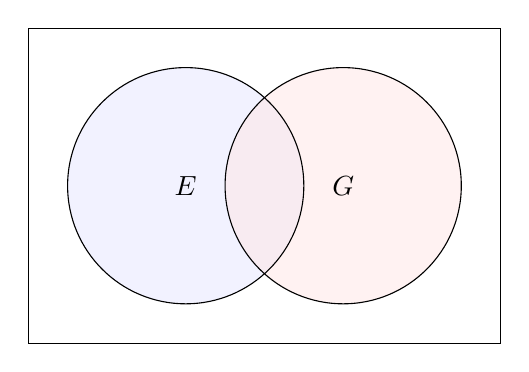
\begin{tikzpicture}

\def\eventE{(2,2) circle (1.5)}
\def\eventG{(4,2) circle (1.5)}

\draw (0,0) rectangle (6,4) node[below left] {$\sS$};

\begin{scope}[fill opacity=0.5]
\fill[blue!10] \eventE;
\fill[red!10] \eventG;
\end{scope}

\draw \eventE node {$E$};
\draw \eventG node {$G$};

\end{tikzpicture}
\repeatcaption{fig:Events E and G}{Events E and G}
\end{figure}
We can see that the area of $E \union G$ is not simply the sum of the areas of $E$ and~$G$. So we have that the probability of $E \union G$ is not simply the sum of the probability of $E$ and $G$. Rather, we must sum the probabilities and subtract the intersection (which gets included twice in the sum) to obtain $P(E \union G)$.
\begin{theorem}
For any events, $A$ and $B$, in a sample space, we have
\[
    P(A \union B) = P(A) + P(B) - P(A \intersect B)
\]
\end{theorem}
\begin{example}
A number between 1 and 6 inclusive is chosen randomly. Let $E = \{\, 2,4,6 \,\}$ be the event the number is odd and let $G = \{\, 4,5,6 \,\}$ be the event that the number is greater than or equal to 4.
\par\smallskip
The probability of the number being even \textbf{or} greater than 4 is $P(E \union G)$. Since both $E$ and~$G$ contain 3~points of the six in the sample space, $P(E) = P(G) = 1/2$. Thus, we can see clearly that $P(E \union G) \neq P(E) + P(G) = 1$ since $\{\, 1 \,\}$ is not in $E$ or $G$ and has a probability of 1/6. Now, note $E \intersect G = \{\, 4,6 \,\}$, so $P(E \intersect G) = 1/3$. We have
\[
    P(E \union G) = P(E) + P(G) - P(E \intersect G) = 1/2 + 1/2 - 1/3 = 2/3
\]
\end{example}
\pagebreak[3]
Now consider the case of the union of three events.\par
\begin{figure}[ht]
\centering
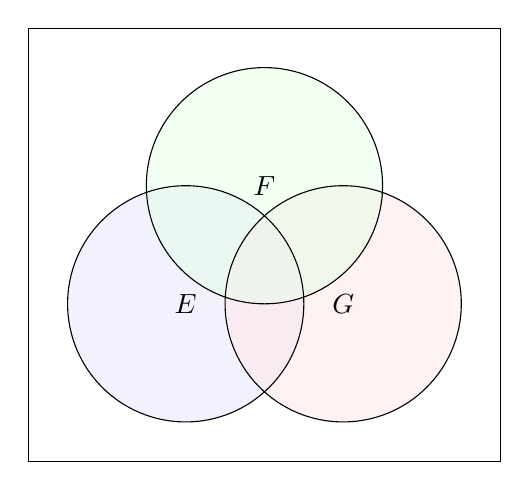
\begin{tikzpicture}

\def\eventE{(2,2) circle (1.5)}
\def\eventG{(4,2) circle (1.5)}
\def\eventF{(3,3.5) circle (1.5)}

\draw (0,0) rectangle (6,5.5) node[below left] {$\sS$};

\begin{scope}[fill opacity=0.5]
\fill[blue!10] \eventE;
\fill[red!10] \eventG;
\fill[green!10] \eventF;
\end{scope}

\draw \eventE node {$E$};
\draw \eventG node {$G$};
\draw \eventF node {$F$};

\end{tikzpicture}
\caption{Three events} \label{fig:Three events}
\end{figure}
Let $A_I$ be the area on the Venn diagram of the event $I$. The area of the union once again is not simply the sum of the areas ($A_E + A_G + A_F$). Instead we can reason out that when we add the three areas we include $A_{E \intersect G}$, $A_{G \intersect F}$, and $A_{F \intersect E}$ twice each and $A_{E \intersect G \intersect F}$ three times. The sum of these doubly counted areas ($A_{E \intersect G} + A_{G \intersect F} + A_{F \intersect E}$) also includes $A_{E \intersect G \intersect F}$ three times. Thus, when we subtract the area of the doubly counted segments, $A_{E \intersect G \intersect F}$ is also subtracted three times leaving this area unaccounted for. Therefore we then add $A_{E \intersect G \intersect F}$ to find the complete area of $E \union G \union F$.
\begin{theorem}
For any events, $A$, $B$ and $C$, in a sample space, we have
\[
    P(A \union B \union C) = P(A) + P(B) + P(C) - P(A \intersect B) - P(B \intersect C) - P(C \intersect A) + P(A \intersect B \intersect C)
\]
\end{theorem}
\subsection*{Mutually Exclusive Events}